% Choose one to switch between slides and handout
\documentclass[]{beamer}
%\documentclass[handout]{beamer}

% Video Meta Data
\title{Bitcoin, Blockchain and Cryptoassets}
\subtitle{Alternative Consensus Protocols}
\author{Prof. Dr. Fabian Schär}
\institute{University of Basel}

% Config File
% Packages
\usepackage[utf8]{inputenc}
\usepackage{hyperref}
\usepackage{gitinfo2}
\usepackage{tikz}
\usepackage{amsmath}
\usepackage{mathtools}
\usepackage{bibentry}
\usepackage{xcolor}
\usepackage{colortbl} % Add colour to LaTeX tables
\usepackage{caption}
\usepackage[export]{adjustbox}
\usepackage{pgfplots} \pgfplotsset{compat = 1.17}
\usepackage{makecell}
\usepackage{fancybox}
\usepackage{ragged2e}
\usepackage{fontawesome}
\usepackage{seqsplit}
\usepackage{tabularx}

% Color Options
\definecolor{highlight}{rgb}{0.65,0.84,0.82}
\definecolor{focus}{rgb}{0.72, 0, 0}
\definecolor{lightred}{rgb}{0.8,0.5,0.5}
\definecolor{midgray}{RGB}{190,195,200}

% Beamer Template Options
\beamertemplatenavigationsymbolsempty
\setbeamertemplate{footline}[frame number]
\setbeamercolor{structure}{fg=black}
\setbeamercolor{footline}{fg=black}
\setbeamercolor{title}{fg=black}
\setbeamercolor{frametitle}{fg=black}
\setbeamercolor{item}{fg=black}
\setbeamercolor{}{fg=black}
\setbeamercolor{bibliography item}{fg=black}
\setbeamercolor*{bibliography entry title}{fg=black}
\setbeamercolor{alerted text}{fg=focus}
\setbeamertemplate{items}[square]
\setbeamertemplate{enumerate items}[default]
\captionsetup[figure]{labelfont={color=black},font={color=black}}
\captionsetup[table]{labelfont={color=black},font={color=black}}

\setbeamertemplate{bibliography item}{\insertbiblabel}

% Link Icon Command
\newcommand{\link}{%
    \tikz[x=1.2ex, y=1.2ex, baseline=-0.05ex]{%
        \begin{scope}[x=1ex, y=1ex]
            \clip (-0.1,-0.1)
                --++ (-0, 1.2)
                --++ (0.6, 0)
                --++ (0, -0.6)
                --++ (0.6, 0)
                --++ (0, -1);
            \path[draw,
                line width = 0.5,
                rounded corners=0.5]
                (0,0) rectangle (1,1);
        \end{scope}
        \path[draw, line width = 0.5] (0.5, 0.5)
            -- (1, 1);
        \path[draw, line width = 0.5] (0.6, 1)
            -- (1, 1) -- (1, 0.6);
        }
    }

% Read Git Data from Github Actions Workflow
% Defaults to gitinfo2 for local builds
\IfFileExists{gitInfo.txt}
	{\input{gitInfo.txt}}
	{
		\newcommand{\gitRelease}{(Local Release)}
		\newcommand{\gitSHA}{\gitHash}
		\newcommand{\gitDate}{\gitAuthorIsoDate}
	}

% Custom Titlepage
\defbeamertemplate*{title page}{customized}[1][]
{
  \vspace{-0cm}\hfill\includegraphics[width=2.5cm]{../config/logo_cif}
  \includegraphics[width=1.9cm]{../config/seal_wwz}
  \\ \vspace{2em}
  \usebeamerfont{title}\textbf{\inserttitle}\par
  \usebeamerfont{title}\usebeamercolor[fg]{title}\insertsubtitle\par  \vspace{1.5em}
  \small\usebeamerfont{author}\insertauthor\par
  \usebeamerfont{author}\insertinstitute\par \vspace{2em}
  \usebeamercolor[fg]{titlegraphic}\inserttitlegraphic
    \tiny \noindent \texttt{Release Ver.: \gitRelease}\\ 
    \texttt{Version Hash: \gitSHA}\\
    \texttt{Version Date: \gitDate}\\ \vspace{1em}
    
    
    \iffalse
  \link \href{https://github.com/cifunibas/Bitcoin-Blockchain-Cryptoassets/blob/main/slides/intro.pdf}
  {Get most recent version}\\
  \link \href{https://github.com/cifunibas/Bitcoin-Blockchain-Cryptoassets/blob/main/slides/intro.pdf}
  {Watch video lecture}\\ 
  
  \fi
  
  \vspace{1em}
  License: \texttt{Creative Commons Attribution-NonCommercial-ShareAlike 4.0 International}\\\vspace{2em}
  \includegraphics[width = 1.2cm]{../config/license}
}


% tikzlibraries
\usetikzlibrary{decorations.pathreplacing}
\usetikzlibrary{decorations.markings}
\usetikzlibrary{positioning}
\usetikzlibrary{calc}
\captionsetup{font=footnotesize}


%%%%%%%%%%%%%%%%%%%%%%%%%%%%%%%%%%%%%%%%%%%%%%
%%%%%%%%%%%%%%%%%%%%%%%%%%%%%%%%%%%%%%%%%%%%%%
\begin{document}
	
	\thispagestyle{empty}
	\begin{frame}[noframenumbering]
		\titlepage
	\end{frame}
	
	
	%%%
	\begin{frame}{Why Consensus Matters}
		Blockchain as \color{focus} chain of transactions and states \color{black} whose \color{focus} compliance with an explicit rule set \color{black} is  attested by a reliable network of record keeping nodes.
		
		\uncover<2->{
			\vspace{1.5 em}
			\textbf{Account statement example:}
			
			\begin{center}
				\begin{tikzpicture}[scale=0.7, every node/.style ={scale=0.8}]
					\input{../assets/figures/account_statement_example}
				\end{tikzpicture}
			\end{center}
			
			\vspace{1 em}
			
			$\Rightarrow$ Value of the chain content depends on the network attesting it.
		}
		
	\end{frame}
	%%%	
	
	%%%
	\begin{frame}{Measures Supporting Consensus}
		
		\textbf{Explicit and unambiguous rule set} for legitimate changes to the ledger and block sequence.
		\vspace{0.25 em}
		
		$\Rightarrow$ Invalid blocks are detected easily and unambiguously.
		\vspace{1.5 em}
		
		\textbf{Decision mechanism} for consensus over different, legitimate extensions of the ledger. 
		\vspace{0.25 em}
		
		$\Rightarrow$ Swiftly resolving situations of uncertainty.
		\vspace{1.5 em}
		
		\textbf{Incentive system} that rewards compliant behaviour and / or penalizes manipulation attempts.
		\vspace{0.25 em}
		
		$\Rightarrow$ Typically in native protocol asset, tying the participant's interest to the sustainable value of the network.
		
	\end{frame}
	%%%
	
	%%%
	\begin{frame}{What Makes a Good Consensus Mechanism?}
		
		Suitability of a consensus mechanism \color{focus} depends on the purpose and usecase \color {black} of a blockchain.
		\vspace{1 em}
		
		\textbf{The Trilemma:}
		
		\begin{center}
			\begin{tikzpicture}[scale=0.6, every node/.style ={scale=0.8}]
				\input{../assets/figures/trilemma}
			\end{tikzpicture}
		\end{center}
		
		\textbf{Generalized Rule:} Subject to tade-offs, i.e., not possible to achieve all three goals. 	
	\end{frame}
	%%%	
	
	%%%
	\begin{frame}{Popular Consensus Mechanisms}
		We will briefly compare the following consensus mechanisms:
		
		\vspace{2.5em}
		
		\centering
		\begin{tikzpicture}[scale=1, every node/.style={scale=1}]
			\begin{footnotesize}
	\coordinate (1) at (-4, 3);
	\coordinate (2) at (0, 3);
	\coordinate (3) at (4, 3);
	
	\node (pow) at (1) {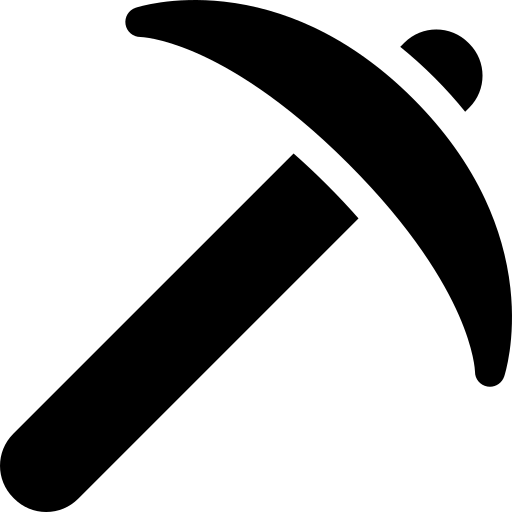
\includegraphics[height = 0.15\textheight]{../assets/images/pickaxe}};
	\node[below = 3pt] at (pow.south) {Proof of Work};
	
	\node (pos) at (2) {
\includegraphics[height = 0.15\textheight]{../assets/images/staking}};
	\node[below = 3pt] at (pos.south) {Proof of Stake};
	
	\node (poa) at (3) {\includegraphics[height = 0.15\textheight]{../assets/images/bank}};
	\node[below = 3pt] at (poa.south) {Proof of Authority};
	
\end{footnotesize}

		\end{tikzpicture}
		
		\pause
		\vspace{1.5em}	
		Openness of the set of consensus-relevant nodes and resources:
		\begin{table}[h]
			\begin{center}
				\begin{tabular}{lccc}
					\hline \hline 
					& Nodes & Resources \\
					\hline
					Proof of Work  &   Open  & Open  \\
					\uncover<3->{Proof of Stake &  Open  & Closed} \\
					\uncover<4->{Proof of Authority  & Closed & Closed}  \\ 
					\hline \hline 
				\end{tabular}
			\end{center}
		\end{table}
	
	\end{frame}
	%%%
	
	%%%
	\begin{frame}{Proof of Work Trilemma}
		\begin{center}
			\begin{tikzpicture}[scale=0.6, every node/.style ={scale=0.8}]
				\input{../assets/figures/trilemma}
			\end{tikzpicture}
		\end{center}
		
		% Menge an resoures open vs closed (resourcen die angreifer braucht)
		\begin{description}[labelwidth=10em]
			\item[\textbf{Scalability}] Every full node needs to process every transaction. Block creation is very resource intensive.
			\item[\textbf{Decentralization}] Open network with many participants. Mining pools compromise decentralization.
			\item[\textbf{Security}] Secured by ressource allocation. Simplicity increases security.
		\end{description}
	\end{frame}
	%%%
	
	%%%
	\begin{frame}{Proof of Stake}
		\small
		To participate in the consensus network, each node - called a validator - needs to \color{focus} deposit and lock native protocol assets\color{black}. This is called staking.
		
		\pause
		\vspace{1.5 em}
		\begin{minipage}{0.2\textwidth}
			\begin{center}
				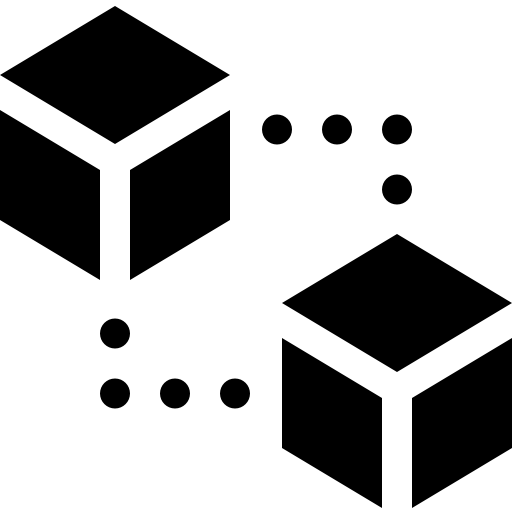
\includegraphics[height=4em]{../assets/images/blocks}
			\end{center}
		\end{minipage}
		\begin{minipage}{0.7\textwidth}
			\textbf{Block creation and transaction validation} \\
			Block creators are selected at random in proportion to their stake. A subset of other validators will then attest to the validity of the created blocks.
		\end{minipage}
	
		\pause
		\vspace{1.5 em}
		\begin{minipage}{0.2\textwidth}
			\begin{center}
				
\includegraphics[height=4em]{../assets/images/mask}
			\end{center}
		\end{minipage}
		\begin{minipage}{0.7\textwidth}
			\textbf{Malicious and unresponsive validators} \\
			Malicious behavior is punished by slashing the staked assets of the offenders. Failure to participate forfeits any rewards and might lead to further punishments.
		\end{minipage}
	
		\pause
		\vspace{1.5 em}
		\begin{minipage}{0.2\textwidth}
			\begin{center}
				
\includegraphics[height=4em]{../assets/images/coin-stack}
			\end{center}
		\end{minipage}
		\begin{minipage}{0.7\textwidth}
			\textbf{Rewards and incentive system} \\
			Validators receive returns on their stake by performing their duties. These rewards are funded by transaction costs and/or newly generated assets.
		\end{minipage}
	\end{frame}
	%%%
	
	%%%
	\begin{frame}{Proof of Stake Trilemma}
		\begin{center}
			\begin{tikzpicture}[scale=0.6, every node/.style ={scale=0.8}]
				\input{../assets/figures/trilemma}
			\end{tikzpicture}
		\end{center}
		
		\begin{description}[labelwidth=10em]
			\item[\textbf{Scalability}] Only a subset of validators need to process each transaction. Proposers are randomly selected.
			\item[\textbf{Decentralization}] Open network with many participants. Potential crowding out over time.
			\item[\textbf{Security}] Pro: Attacker must acquire protocol asset.\\ Con: Complex design may introduce new attack vectors.
		\end{description}
	\end{frame}
	%%%
	
	%%%
	\begin{frame}{Proof of Authority}
		\small
		The consensus network consists of a \color{focus}small set of approved nodes \color{black} - called validators. They are identified and therefore have their reputation at stake.
		
		\pause
		\vspace{1.5 em}
		\begin{minipage}{0.2\textwidth}
			\begin{center}
				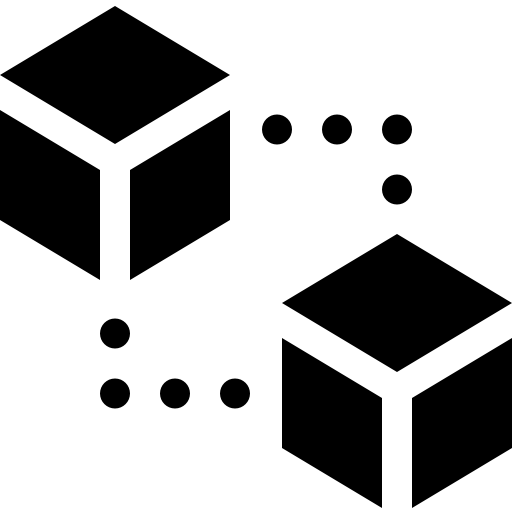
\includegraphics[height=4em]{../assets/images/blocks}
			\end{center}
		\end{minipage}
		\begin{minipage}{0.7\textwidth}
			\textbf{Block creation and transaction validation} \\
			Validators (alternating or random selection) create and validate blocks. Other validators will attest to the validity of the created blocks.
		\end{minipage}
		
		\pause
		\vspace{1.5 em}
		\begin{minipage}{0.2\textwidth}
			\begin{center}
				
\includegraphics[height=4em]{../assets/images/mask}
			\end{center}
		\end{minipage}
		\begin{minipage}{0.7\textwidth}
			\textbf{Malicious and unresponsive validators} \\
			Malicious or unresponsive behavior is punished by exclusion, tarnished reputation and potential legal actions.
		\end{minipage}
		
		\pause
		\vspace{1.5 em}
		\begin{minipage}{0.2\textwidth}
			\begin{center}
				
\includegraphics[height=4em]{../assets/images/coin-stack}
			\end{center}
		\end{minipage}
		\begin{minipage}{0.7\textwidth}
			\textbf{Rewards and incentive system} \\
			Block rewards are usually limited to the transaction costs. Validators often have external incentives to run their nodes.
		\end{minipage}
	\end{frame}
	%%%
	
	%%%
	\begin{frame}{Proof of Authority Trilemma}
		\begin{center}
			\begin{tikzpicture}[scale=0.6, every node/.style ={scale=0.8}]
				\input{../assets/figures/trilemma}
			\end{tikzpicture}
		\end{center}
		
		\begin{description}[labelwidth=10em]
			\item[\textbf{Scalability}] Very small set of validators and simple mechanism. Higher ceiling for validator performance (hardware).
			\item[\textbf{Decentralization}] Closed network with risk of collusion. In many cases: heavily centralized. 
			\item[\textbf{Security}] Not immutable (with all pros and cons).\\ In many cases: Just your average database.
		\end{description}
	\end{frame}
	%%%
	
	%%%
	\begin{frame}{Key Takeaways}
		\begin{enumerate}
			\item All consensus algorithms have their pros and cons. 
			\item<2-> Immutability and transparency is not just given, because you call your project ``Blockchain'' -- it depends on the architecture, and in particular, on the choice of the consensus mechanism.
			\item<3-> It is possible for a blockchain to change its consensus mechanism via a hard fork.	
			\item<4-> These are just a few high level examples to give you an overview. There are hundreds of variations and other consensus mechanisms.
		\end{enumerate}
	\end{frame}
	%%%
	
\end{document}